%!TeX root=../sensetop.tex
\chapter[Chapter \thechapter]{}
\lettrine[lraise=0.3]{M}{arianne}'s preserver, as Margaret, with more elegance than precision, styled Willoughby, called at the cottage early the next morning to make his personal enquiries. He was received by Mrs Dashwood with more than politeness; with a kindness which Sir John's account of him and her own gratitude prompted; and every thing that passed during the visit tended to assure him of the sense, elegance, mutual affection, and domestic comfort of the family to whom accident had now introduced him. Of their personal charms he had not required a second interview to be convinced.

Miss Dashwood had a delicate complexion, regular features, and a remarkably pretty figure. Marianne was still handsomer. Her form, though not so correct as her sister's, in having the advantage of height, was more striking; and her face was so lovely, that when in the common cant of praise, she was called a beautiful girl, truth was less violently outraged than usually happens. Her skin was very brown, but, from its transparency, her complexion was uncommonly brilliant; her features were all good; her smile was sweet and attractive; and in her eyes, which were very dark, there was a life, a spirit, an eagerness, which could hardly be seen without delight. From Willoughby their expression was at first held back, by the embarrassment which the remembrance of his assistance created. But when this passed away, when her spirits became collected, when she saw that to the perfect good-breeding of the gentleman, he united frankness and vivacity, and above all, when she heard him declare, that of music and dancing he was passionately fond, she gave him such a look of approbation as secured the largest share of his discourse to herself for the rest of his stay.

It was only necessary to mention any favourite amusement to engage her to talk. She could not be silent when such points were introduced, and she had neither shyness nor reserve in their discussion. They speedily discovered that their enjoyment of dancing and music was mutual, and that it arose from a general conformity of judgment in all that related to either. Encouraged by this to a further examination of his opinions, she proceeded to question him on the subject of books; her favourite authors were brought forward and dwelt upon with so rapturous a delight, that any young man of five and twenty must have been insensible indeed, not to become an immediate convert to the excellence of such works, however disregarded before. Their taste was strikingly alike. The same books, the same passages were idolized by each—or if any difference appeared, any objection arose, it lasted no longer than till the force of her arguments and the brightness of her eyes could be displayed. He acquiesced in all her decisions, caught all her enthusiasm; and long before his visit concluded, they conversed with the familiarity of a long-established acquaintance.

<Well, Marianne,> said Elinor, as soon as he had left them, <for \textit{one} morning I think you have done pretty well. You have already ascertained Mr Willoughby's opinion in almost every matter of importance. You know what he thinks of Cowper and Scott; you are certain of his estimating their beauties as he ought, and you have received every assurance of his admiring Pope no more than is proper. But how is your acquaintance to be long supported, under such extraordinary despatch of every subject for discourse? You will soon have exhausted each favourite topic. Another meeting will suffice to explain his sentiments on picturesque beauty, and second marriages, and then you can have nothing farther to ask.>

<Elinor,> cried Marianne, <is this fair? is this just? are my ideas so scanty? But I see what you mean. I have been too much at my ease, too happy, too frank. I have erred against every common-place notion of decorum; I have been open and sincere where I ought to have been reserved, spiritless, dull, and deceitful—had I talked only of the weather and the roads, and had I spoken only once in ten minutes, this reproach would have been spared.>

<My love,> said her mother, <you must not be offended with Elinor—she was only in jest. I should scold her myself, if she were capable of wishing to check the delight of your conversation with our new friend.> Marianne was softened in a moment.

Willoughby, on his side, gave every proof of his pleasure in their acquaintance, which an evident wish of improving it could offer. He came to them every day. To enquire after Marianne was at first his excuse; but the encouragement of his reception, to which every day gave greater kindness, made such an excuse unnecessary before it had ceased to be possible, by Marianne's perfect recovery. She was confined for some days to the house; but never had any confinement been less irksome. Willoughby was a young man of good abilities, quick imagination, lively spirits, and open, affectionate manners. He was exactly formed to engage Marianne's heart, for with all this, he joined not only a captivating person, but a natural ardour of mind which was now roused and increased by the example of her own, and which recommended him to her affection beyond every thing else.

His society became gradually her most exquisite enjoyment. They read, they talked, they sang together; his musical talents were considerable; and he read with all the sensibility and spirit which Edward had unfortunately wanted.

% \begin{figure}[tbph]
% \centering
% 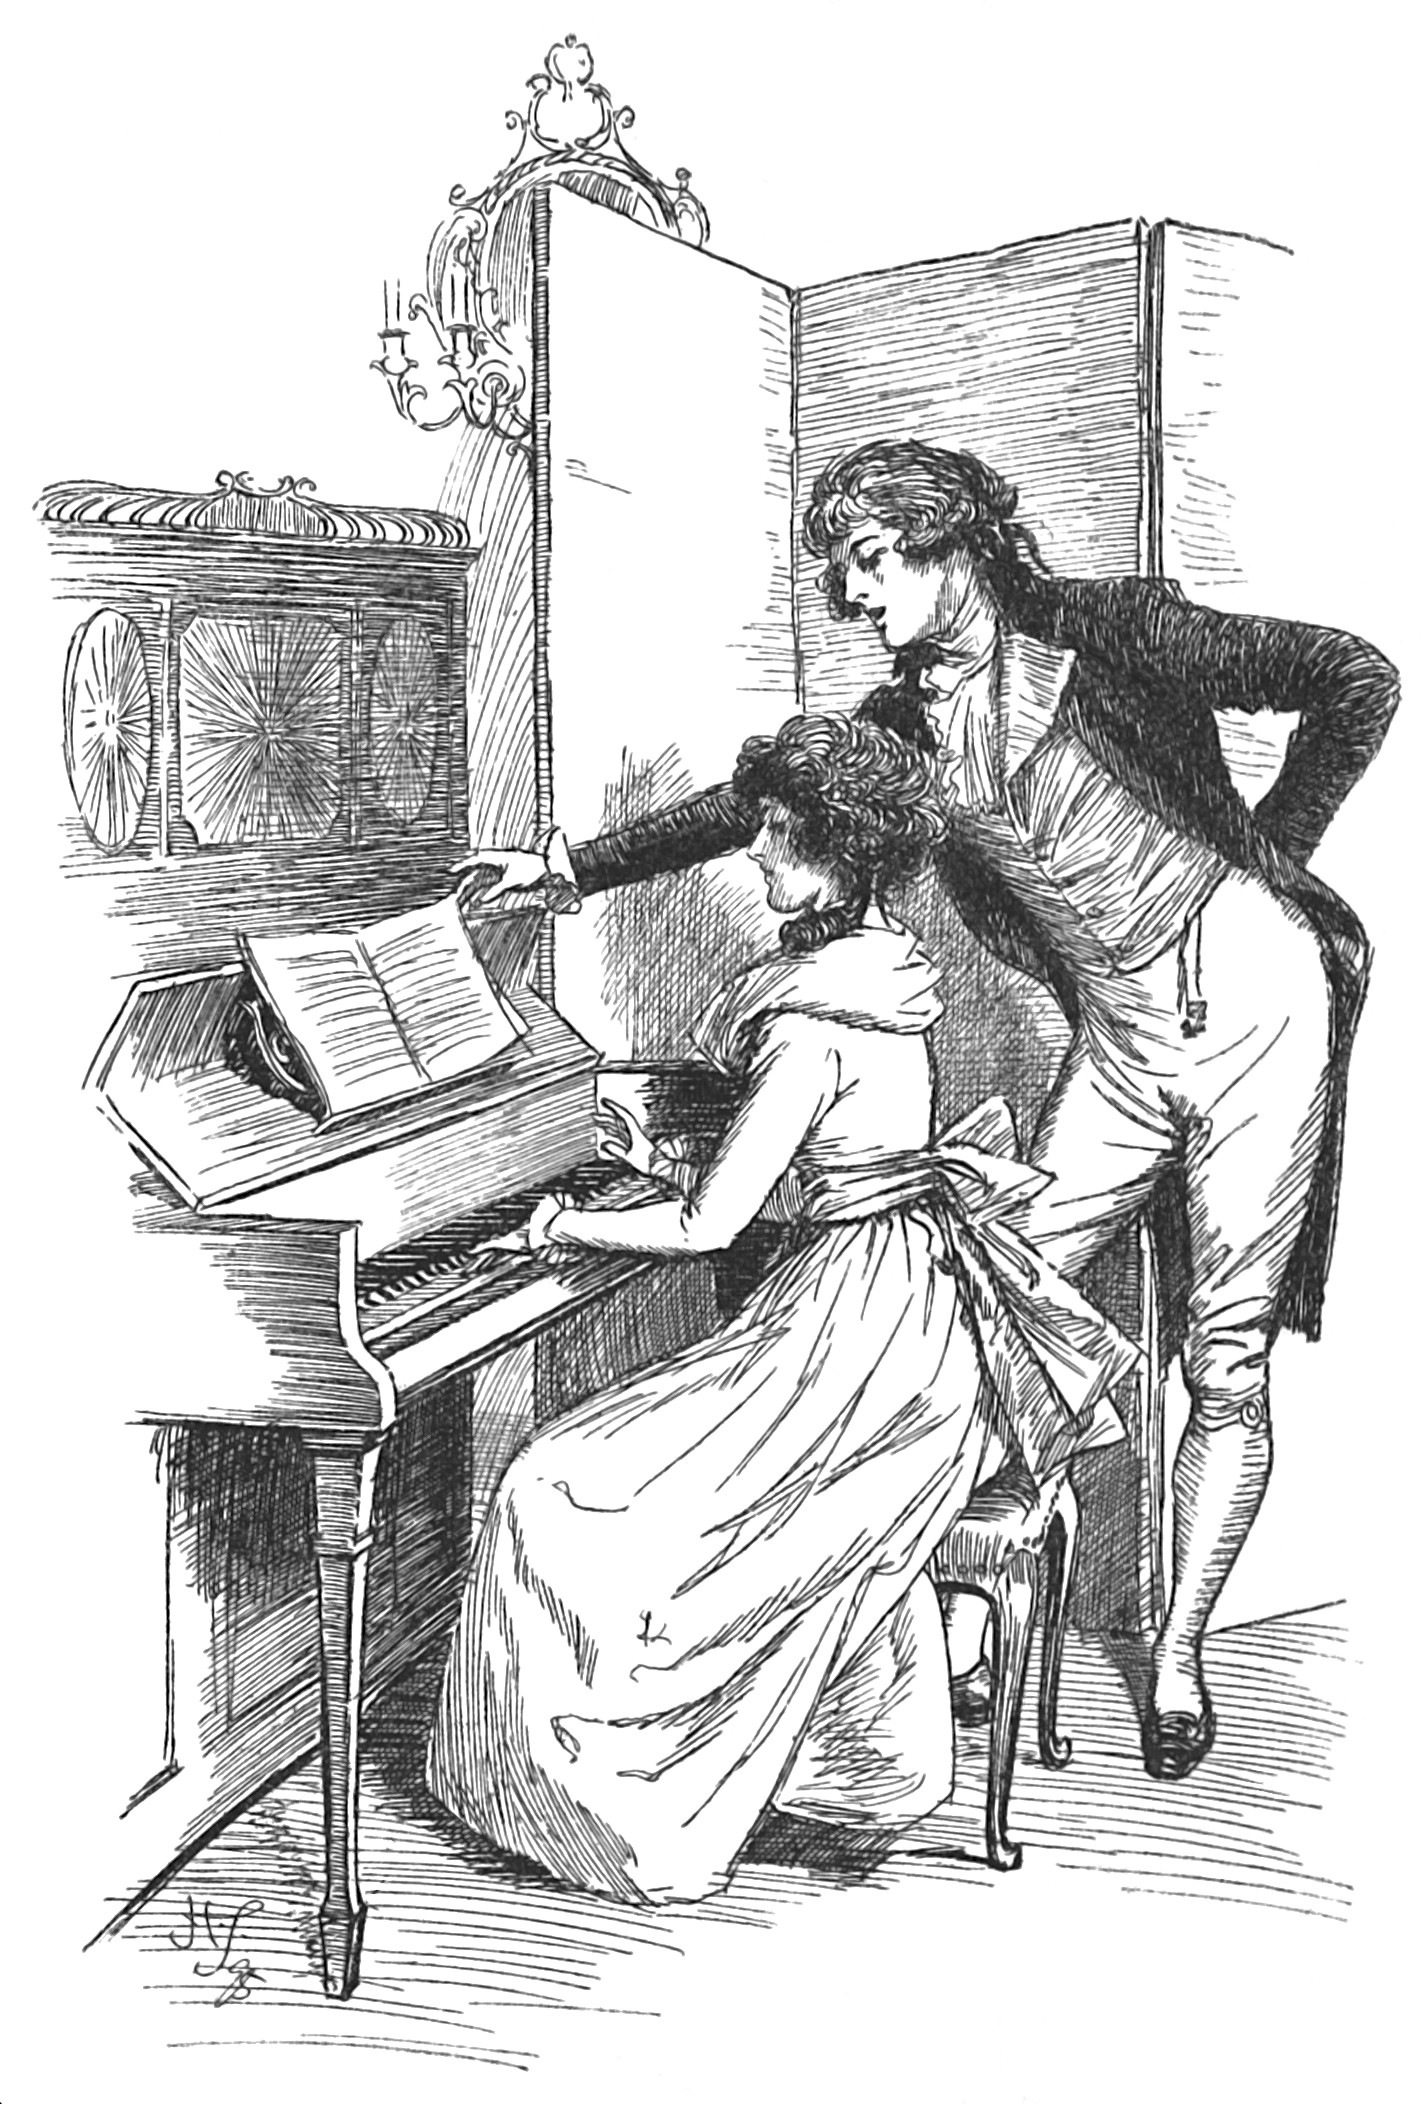
\includegraphics[width=\linewidth]{10sang}
% \caption{They sang together}
% \end{figure}

\begin{bwbigpic}
	[1.0]
	{10sang} 
	{They sang together} 
\end{bwbigpic}

In Mrs Dashwood's estimation he was as faultless as in Marianne's; and Elinor saw nothing to censure in him but a propensity, in which he strongly resembled and peculiarly delighted her sister, of saying too much what he thought on every occasion, without attention to persons or circumstances. In hastily forming and giving his opinion of other people, in sacrificing general politeness to the enjoyment of undivided attention where his heart was engaged, and in slighting too easily the forms of worldly propriety, he displayed a want of caution which Elinor could not approve, in spite of all that he and Marianne could say in its support.

Marianne began now to perceive that the desperation which had seized her at sixteen and a half, of ever seeing a man who could satisfy her ideas of perfection, had been rash and unjustifiable. Willoughby was all that her fancy had delineated in that unhappy hour and in every brighter period, as capable of attaching her; and his behaviour declared his wishes to be in that respect as earnest, as his abilities were strong.

Her mother too, in whose mind not one speculative thought of their marriage had been raised, by his prospect of riches, was led before the end of a week to hope and expect it; and secretly to congratulate herself on having gained two such sons-in-law as Edward and Willoughby.

Colonel Brandon's partiality for Marianne, which had so early been discovered by his friends, now first became perceptible to Elinor, when it ceased to be noticed by them. Their attention and wit were drawn off to his more fortunate rival; and the raillery which the other had incurred before any partiality arose, was removed when his feelings began really to call for the ridicule so justly annexed to sensibility. Elinor was obliged, though unwillingly, to believe that the sentiments which Mrs Jennings had assigned him for her own satisfaction, were now actually excited by her sister; and that however a general resemblance of disposition between the parties might forward the affection of Mr Willoughby, an equally striking opposition of character was no hindrance to the regard of Colonel Brandon. She saw it with concern; for what could a silent man of five and thirty hope, when opposed to a very lively one of five and twenty? and as she could not even wish him successful, she heartily wished him indifferent. She liked him—in spite of his gravity and reserve, she beheld in him an object of interest. His manners, though serious, were mild; and his reserve appeared rather the result of some oppression of spirits than of any natural gloominess of temper. Sir John had dropped hints of past injuries and disappointments, which justified her belief of his being an unfortunate man, and she regarded him with respect and compassion.

Perhaps she pitied and esteemed him the more because he was slighted by Willoughby and Marianne, who, prejudiced against him for being neither lively nor young, seemed resolved to undervalue his merits.

<Brandon is just the kind of man,> said Willoughby one day, when they were talking of him together, <whom every body speaks well of, and nobody cares about; whom all are delighted to see, and nobody remembers to talk to.>

<That is exactly what I think of him,> cried Marianne.

<Do not boast of it, however,> said Elinor, <for it is injustice in both of you. He is highly esteemed by all the family at the park, and I never see him myself without taking pains to converse with him.>

<That he is patronised by \textit{you},> replied Willoughby, <is certainly in his favour; but as for the esteem of the others, it is a reproach in itself. Who would submit to the indignity of being approved by such a woman as Lady Middleton and Mrs Jennings, that could command the indifference of any body else?>

<But perhaps the abuse of such people as yourself and Marianne will make amends for the regard of Lady Middleton and her mother. If their praise is censure, your censure may be praise, for they are not more undiscerning, than you are prejudiced and unjust.>

<In defence of your \textit{protégé} you can even be saucy.>

<My \textit{protégé}, as you call him, is a sensible man; and sense will always have attractions for me. Yes, Marianne, even in a man between thirty and forty. He has seen a great deal of the world; has been abroad, has read, and has a thinking mind. I have found him capable of giving me much information on various subjects; and he has always answered my inquiries with readiness of good-breeding and good nature.>

<That is to say,> cried Marianne contemptuously, <he has told you, that in the East Indies the climate is hot, and the mosquitoes are troublesome.>

<He \textit{would} have told me so, I doubt not, had I made any such inquiries, but they happened to be points on which I had been previously informed.>

<Perhaps,> said Willoughby, <his observations may have extended to the existence of nabobs, gold mohrs, and palanquins.>

<I may venture to say that \textit{his} observations have stretched much further than \textit{your} candour. But why should you dislike him?>

<I do not dislike him. I consider him, on the contrary, as a very respectable man, who has every body's good word, and nobody's notice; who has more money than he can spend, more time than he knows how to employ, and two new coats every year.>

<Add to which,> cried Marianne, <that he has neither genius, taste, nor spirit. That his understanding has no brilliancy, his feelings no ardour, and his voice no expression.>

<You decide on his imperfections so much in the mass,> replied Elinor, <and so much on the strength of your own imagination, that the commendation \textit{I} am able to give of him is comparatively cold and insipid. I can only pronounce him to be a sensible man, well-bred, well-informed, of gentle address, and, I believe, possessing an amiable heart.>

<Miss Dashwood,> cried Willoughby, <you are now using me unkindly. You are endeavouring to disarm me by reason, and to convince me against my will. But it will not do. You shall find me as stubborn as you can be artful. I have three unanswerable reasons for disliking Colonel Brandon; he threatened me with rain when I wanted it to be fine; he has found fault with the hanging of my curricle, and I cannot persuade him to buy my brown mare. If it will be any satisfaction to you, however, to be told, that I believe his character to be in other respects irreproachable, I am ready to confess it. And in return for an acknowledgment, which must give me some pain, you cannot deny me the privilege of disliking him as much as ever.>